\section{Quantile-Quantile Plot \cite{wiki-q-q-plot}}\label{Quantile-Quantile Plot}
A Q–Q plot (quantile–quantile plot) is a probability plot, a graphical method for comparing two probability distributions by plotting their quantiles against each other. A point (x, y) on the plot corresponds to one of the quantiles of the second distribution (y-coordinate) plotted against the same quantile of the first distribution (x-coordinate). This defines a parametric curve where the parameter is the index of the quantile interval.

\begin{table}[H]
    \begin{minipage}{0.45\textwidth}
        \begin{figure}[H]
            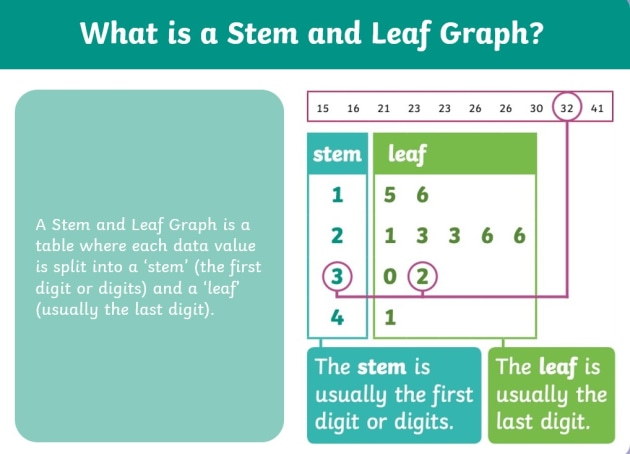
\includegraphics[height=5cm]{Pictures/data/data_stem-and-leaf-plot.jpg}
            \caption{Graph: Stem \& Leaf Plot}
        \end{figure}
    \end{minipage}
    \hfill
    \begin{minipage}{0.45\textwidth}
        \begin{figure}[H]
            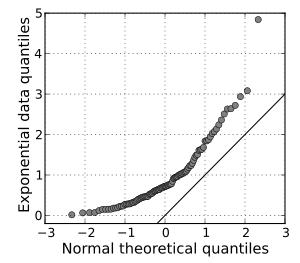
\includegraphics[height=5cm]{Pictures/data/data_q_q_plot.png}
            \caption{Graph: Quantile–Quantile (Q–Q) plot}
        \end{figure}
    \end{minipage}
\end{table}
